%% main.tex - adapted from reference-template (title page and style preserved)
%% Author updated to user's name
\documentclass[a4paper,12pt]{report}
\usepackage[utf8]{inputenc}
\usepackage[T1]{fontenc}
\usepackage[spanish]{babel}
\usepackage{acronym}
\usepackage{amsfonts}
\usepackage{amsmath}
\usepackage{amssymb}
\usepackage{array}
\usepackage{caption}
\usepackage{enumitem}
\usepackage{fancyhdr}
\usepackage{float}
\usepackage{geometry}
\usepackage{graphicx}
\usepackage{hyperref}
\usepackage{indentfirst}
\usepackage{lmodern}
\usepackage{longtable}
\usepackage{makecell}
\usepackage{microtype}
\usepackage[nottoc]{tocbibind}
\usepackage{siunitx}
\usepackage{titlesec}
\usepackage{url}
\usepackage{csquotes}
\usepackage{subcaption}
\usepackage{booktabs}
\usepackage{tikz}
\usetikzlibrary{positioning, babel}
\usepackage{listings}
\usepackage{setspace}
\usepackage{apacite}
\usepackage{parskip} % Added for extra line between paragraphs

% Geometry and title formatting
\geometry{top=3cm,bottom=3cm,left=3cm,right=3cm}
\titleformat{\chapter}[display]{\normalfont\huge\bfseries}{\chaptertitlename\ \thechapter}{20pt}{\Huge}
\titlespacing*{\chapter}{0pt}{-30pt}{20pt}
\titleformat{\section}[block]{\normalfont\Large\bfseries}{\thesection}{1em}{}
\titleformat{\subsection}[block]{\normalfont\large\bfseries}{\thesubsection}{1em}{}

\numberwithin{equation}{chapter}
\numberwithin{figure}{chapter}
\numberwithin{table}{chapter}

\pagestyle{fancy}
\fancyhf{}
\cfoot{\thepage}

% Project metadata
\newcommand{\titulo}{Benchmarking de m\'etodos de reducci\'on de ruido en im\'agenes simuladas DC2 del Vera Rubin Observatory}
\newcommand{\autor}{Jheison Martinez Bolivar}
\newcommand{\codigo}{}
\newcommand{\programa}{Maestr\'ia en Inteligencia Artificial}
\newcommand{\universidad}{Universidad La Salle}
\newcommand{\correo}{jhmartinez07@unisalle.edu.co}

\hypersetup{pdfauthor={\autor},pdftitle={\titulo},pdfsubject={\programa},pdfkeywords={astro, denoising, Rubin Observatory},colorlinks=true,linkcolor=black,citecolor=black,urlcolor=black}

\begin{document}

\begin{titlepage}
    \centering\vspace*{\fill}
    % show La Salle logo if provided, otherwise fallback to project image
    \IfFileExists{assets/images/logosalle.png}{
\includegraphics[width=8cm]{assets/images/logosalle.png}\\[1cm]}{\IfFileExists{assets/images/xfm8rUJf1h.png}{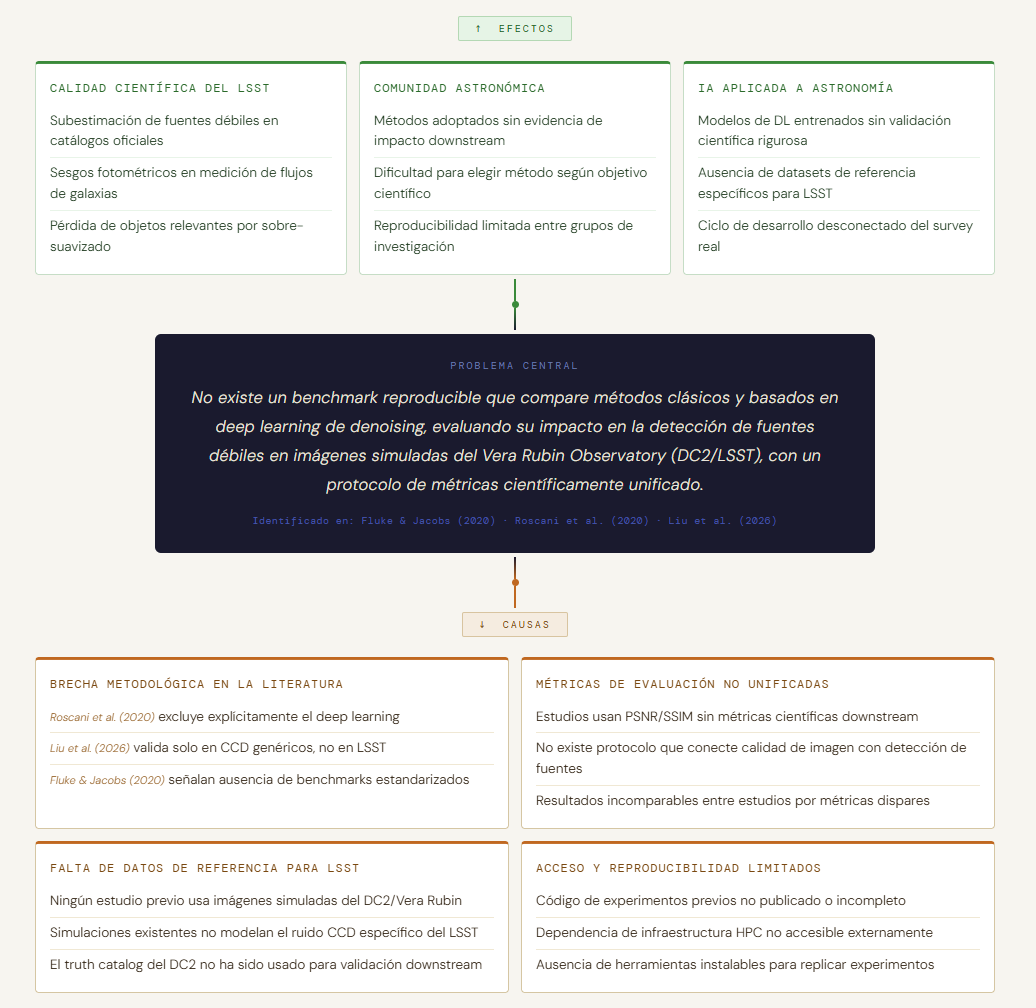
\includegraphics[width=8cm]{assets/images/xfm8rUJf1h.png}\\[1cm]}{}}
    \universidad\\[0.5cm]\programa\\[2cm]
    {\LARGE\bfseries \titulo}\\[2cm]
    \textbf{Propuesta de Proyecto}\\[2cm]
    {\Large \autor}
    \par
    {\codigo}
    \par\vspace{1cm}
    \correo
    \par\vspace{2cm}
    Fecha de entrega: \today
    \par\vspace{1cm}
    \vspace*{\fill}
\end{titlepage}

  \thispagestyle{empty}\newpage

  % Resumen (use modular file)
\chapter*{Resumen}\addcontentsline{toc}{chapter}{Resumen}

Este borrador presenta el estado actual del proyecto ``Astro Denoise Benchmark'' y documenta el alcance hasta el estado del arte y los datos preliminares. Se describen el contexto cient\'ifico, la motivaci\'on inspiracional para una ciencia m\'as abierta y transparente, el planteamiento del problema y los datasets DC2 que se usar\'an para evaluaci\'on. Adem\'as, se documenta el procedimiento reproducible de selecci\'on bibliogr\'afica potenciado por aprendizaje activo y la integraci\'on inicial de referencias clave que definen el panorama actual del denoising astron\'omico.

El objetivo del documento es ofrecer una base t\'ecnicamente s\'olida y reproducible para comparar m\'etodos de denoising (enfoc\'andose en BM3D y U-Net) mediante m\'etricas orientadas a la ciencia \textemdash completitud y pureza\textemdash en im\'agenes simuladas del Vera Rubin Observatory (DC2). Este informe no contiene a\'un resultados experimentales finales: presenta el alcance, los datos disponibles y la metodolog\'ia propuesta para las pr\'oximas etapas del benchmark.

Se han versionado los scripts, los datos y las fichas bibliogr\'aficas para facilitar la auditor\'ia y la repetici\'on del estudio por parte de la comunidad cient\'ifica.

\bigskip

\textbf{Palabras clave:} denoising; im\'agenes astron\'omicas; DC2; BM3D; U-Net; completitud; pureza; Vera Rubin Observatory; reproducibilidad.

\bigskip

\textbf{Keywords:} denoising; astronomical images; DC2; BM3D; U-Net; completeness; purity; Vera Rubin Observatory; reproducibility.


  % Table of contents and lists (compact)
\tableofcontents\thispagestyle{empty}
  \listoffigures\thispagestyle{empty}

  % Chapters (modular)
\chapter{Contexto y Motivaci\'on}

El proyecto ``Astro Denoise'' nace de la necesidad de evaluar, con rigor cient\'ifico, c\'omo las t\'ecnicas modernas de restauraci\'on de im\'agenes afectan la capacidad de las encuestas astron\'omicas para descubrir y caracterizar objetos tenues. El Vera Rubin Observatory (LSST) representa una revoluci\'on en volumen y profundidad de datos: detectar señales d\'ebiles en im\'agenes coadded es cr\'itico para objetivos como cosmolog\'ia de precisi\'on, mapeo de la V\'ia L\'actea, descubrimiento de objetos transitorios y estudios del Sistema Solar. Mejorar la relaci\'on señal\textendash ruido sin introducir sesgos es, por tanto, una prioridad cient\'ifica.

Este proyecto integra dos dimensiones esenciales: (1) rigor metodol\'ogico \textemdash protocolos reproducibles, m\'etricas cient\'ificas y control de semillas/random states\textemdash y (2) relevancia cient\'ifica \textemdash medir el impacto de la reducci\'on de ruido sobre la capacidad de detecci\'on y la calidad fotom\'etrica en cat\'alogos que alimentan an\'alisis astrof\'isicos. En otras palabras, no se persigue la m\'axima mejora perceptual, sino la mejora cuantificable y verificable en m\'etricas que importan para la ciencia.

La elecci\'on del conjunto de datos (DC2 dr6\textendash v4) y la atenci\'on a reproducibilidad responden a las recomendaciones de la comunidad y a los objetivos cient\'ificos del Rubin Observatory \cite{objetivos_rubin_2024}, que enfatizan descubrimientos estad\'isticos, trazabilidad de an\'alisis y estimaci\'on rigurosa de incertidumbres instrumentales.

Motivaci\'on inspiracional: este trabajo pretende acelerar descubrimientos al reducir las barreras t\'ecnicas que impiden detectar y medir fuentes d\'ebiles. Al construir un benchmark modular, reproducible y abierto, se facilita la comparaci\'on objetiva entre m\'etodos cl\'asicos y de IA, promoviendo buenas pr\'acticas de ciencia de datos en astronom\'ia. El impacto potencial incluye: mejores cat\'alogos para cosmolog\'ia y astrof\'isica, pipelines reutilizables para futuras encuestas y un marco de evaluaci\'on que favorece transparencia, reproducibilidad y colaboraci\'on abierta.

Se resalta la importancia de documentar cada decisi\'on \textemdash desde criterios de selecci\'on bibliogr\'afica hasta preprocesado y par\'ametros del detector\textemdash para que los resultados sean auditables y replicables por cualquier equipo de la comunidad.

\chapter{Planteamiento del problema}

\section{Pregunta de investigaci\'on}

\textquestiondown C\'omo afectan las t\'ecnicas modernas de restauraci\'on de im\'agenes a la capacidad de las observaciones astron\'omicas para descubrir y caracterizar objetos tenues, y c\'omo pueden evaluarse de manera reproducible y cient\'ificamente v\'alida?

\section{Objetivos}

\subsection{Objetivo general}

Desarrollar una plataforma de benchmarking reproducible que compare m\'etodos de reducci\'on de ruido en im\'agenes simuladas DC2 del Vera Rubin Observatory, evaluando en cada m\'etodo la recuperaci\'on de fuentes d\'ebiles, la calidad de imagen resultante y su coste computacional.

\subsection{Objetivos espec\'ificos}

Los objetivos espec\'ificos se presentan en el orden cronol\'ogico en que se cumplen.

\begin{enumerate}
  \item Implementar un ecosistema modular y extensible con un protocolo com\'un de l\'inea de comandos, en el que cada m\'etodo de reducci\'on de ruido (BM3D y U-Net, junto con una condici\'on de control sin procesamiento) se empaquete de forma independiente con su propio entorno y se comunique con un orquestador mediante una interfaz fija (imagen FITS de entrada y de salida, metadatos en JSON), de modo que un m\'etodo nuevo pueda incorporarse sin modificar el orquestador.
  \item Establecer m\'etricas confiables para evaluar la recuperaci\'on de fuentes, basadas en el cruce uno a uno de las detecciones con el cat\'alogo de verdad de DC2 (completitud, pureza, completitud en funci\'on de la magnitud y precisi\'on fotom\'etrica) y complementadas con m\'etricas de calidad de imagen (PSNR, SSIM y ruido de fondo), verificando cada c\'alculo contra su definici\'on en al menos dos fuentes independientes de la literatura.
  \item Proporcionar herramientas de medici\'on del coste computacional de cada m\'etodo (tiempo de ejecuci\'on por regi\'on, memoria m\'axima utilizada y regiones procesadas por unidad de tiempo), tomadas desde fuera del proceso del m\'etodo para que se apliquen por igual a cualquier implementaci\'on y reportadas junto con la descripci\'on del equipo en que se ejecutaron.
  \item Desarrollar los m\'etodos de reducci\'on de ruido evaluados, BM3D como representante de los m\'etodos cl\'asicos y una U-Net como representante del aprendizaje profundo, integrados al ecosistema. La U-Net se entrena exclusivamente con regiones de DC2 no declaradas en el conjunto de evaluaci\'on, y su receta de entrenamiento y sus pesos se publican junto con el m\'etodo.
  \item Crear un benchmark reproducible sobre un conjunto de datos curado y versionado a partir de DESC DC2, compuesto por regiones multibanda tomadas de varias zonas del cielo con su cat\'alogo de verdad. Cada versi\'on del conjunto se identifica por checksums y declara expl\'icitamente las regiones del cielo que incluye, de modo que todo resultado se reporte contra una versi\'on concreta. La reproducibilidad se entiende como la obtenci\'on de las mismas m\'etricas cient\'ificas al repetir la ejecuci\'on con la misma versi\'on de datos y de c\'odigo.
\end{enumerate}

\section{\'Arbol de problemas}

A continuaci\'on se presenta el an\'alisis causal enriquecido, con una distribuci\'on sim\'etrica de factores:

\begin{figure}[H]
  \centering
  \shorthandoff{>}
  \resizebox{\textwidth}{!}{
    \begin{tikzpicture}[
      node distance=1.2cm and 0.4cm,
      every node/.style={font=\small, align=center, line width=0.5pt},
      effect/.style={rectangle, fill=gray!5, draw=gray!50, text width=3.9cm, minimum height=1.6cm, rounded corners=1pt},
      problem/.style={rectangle, fill=gray!85, draw=gray!90, text=white, text width=11.5cm, font=\small\bfseries, minimum height=1.8cm, rounded corners=1pt},
      cause/.style={rectangle, fill=gray!15, draw=gray!60, text width=3.8cm, minimum height=1.6cm, rounded corners=1pt},
      connector/.style={draw=gray!70, thick, -latex},
      labelnode/.style={font=\small\scshape\bfseries, text=black!60}
    ]

    % Problema Central
    \node[problem] (core) at (0,0)
      {Ausencia de un marco de evaluaci\'on independiente y reproducible que priorice m\'etricas de integridad cient\'ifica (completitud y pureza) sobre la est\'etica visual en im\'agenes del Rubin Observatory};

    % Efectos (Arriba)
    \node[effect, above=of core] (e2)
      {\textsc{Barrera de Confianza}\\Desconfianza en modelos IA ``black-box'' sin validaci\'on externa sistem\'atica.};
    \node[effect, left=of e2] (e1)
      {\textsc{Sesgos Cosmol\'ogicos}\\Alteraci\'on de medidas de elipticidad y flujo d\'ebil (Weak Lensing).};
    \node[effect, right=of e2] (e3)
      {\textsc{Ineficiencia T\'ecnica}\\Adopci\'on de m\'etodos costosos sin beneficio probado en tareas downstream.};

    % Label efectos — above=of usa el bounding box real, no minimum height
    \node[labelnode, above=0.5cm of e2]
      {$\uparrow$ Efectos del Problema $\uparrow$};

    % Causas (Abajo)
    \node[cause] (c1) at (-6.4,-3.2)
      {\textsc{Sesgo de Autovalidaci\'on}\\Investigadores validan sus modelos con marcos ad-hoc no estandarizados.};
    \node[cause] (c2) at (-2.1,-3.2)
      {\textsc{M\'etricas Insuficientes}\\Uso predominante de PSNR/SSIM que ignoran la fidelidad fotom\'etrica.};
    \node[cause] (c3) at (2.1,-3.2)
      {\textsc{Opacidad Algor\'itmica}\\Falta de pipelines abiertos, semillas y pesos compartidos.};
    \node[cause] (c4) at (6.4,-3.2)
      {\textsc{Desconexi\'on con DC2}\\Dificultad para integrar el Truth Catalog en la validaci\'on masiva.};

    % Label causas
    \node[labelnode] at (0,-5.4)
      {$\downarrow$ Causas Ra\'iz $\downarrow$};

    % Conectores Efectos
    \draw[connector] (core.north) -- +(0,0.5) -| (e1.south);
    \draw[connector] (core.north) -- +(0,0.5) -- (e2.south);
    \draw[connector] (core.north) -- +(0,0.5) -| (e3.south);

    % Conectores Causas
    \draw[connector] (c1.north) |- +(0,0.6) -| (core.south);
    \draw[connector] (c2.north) |- +(0,0.6) -| (core.south);
    \draw[connector] (c3.north) |- +(0,0.6) -| (core.south);
    \draw[connector] (c4.north) |- +(0,0.6) -| (core.south);

    \end{tikzpicture}
  }
  \shorthandon{>}
  \caption{\'Arbol de problemas enriquecido: factores que impiden la validaci\'on objetiva del denoising astron\'omico.}
\end{figure}
\chapter{Estado del arte}

\section{Panorama general}

El estado del arte en reducci\'on de ruido en im\'agenes astron\'omicas muestra un desplazamiento claro desde m\'etodos cl\'asicos (wavelets, variacionales, priors expl\'icitos) hacia arquitecturas profundas con modelado probabil\'istico (U-Net, Transformers y difusi\'on), pero con una tensi\'on metodol\'ogica persistente: mejorar la calidad visual no garantiza preservar la validez cient\'ifica de la inferencia downstream \cite{elad2023revolution, vojtekova2020unet, shirasaki2021noise, akhaury2025joint, guo2026detection}.

En este trabajo, el foco no es presentar otro m\'etodo aislado de reducci\'on de ruido, sino consolidar una base comparativa reproducible para LSST/DC2 donde la evaluaci\'on se centre en impacto cient\'ifico medible (detecci\'on, fotometr\'ia, forma, sesgo) y no solo en fidelidad perceptual.

\section{Proceso de cribado y s\'intesis (PRISMA + RAG)}

La revisi\'on se reconstruy\'o de forma transparente sobre un corpus inicial de 304 PDFs, combinando aprendizaje activo (ASReview), re-ranqueo sem\'antico con RAG y verificaci\'on manual de metadatos en PDF. El uso de RAG se limit\'o a priorizaci\'on y trazabilidad sem\'antica de relaciones complejas (m\'etricas, tareas, sesgos), mientras que la decisi\'on final de inclusi\'on/exclusi\'on fue auditada manualmente.

\begin{mermaid}[width=0.95\linewidth, caption={Diagrama PRISMA del cribado (corpus astron\'omico de reducci\'on de ruido)}, pos=t]
flowchart TD
    A[Registros identificados\\nPDFs recuperados: n = 304]
    B[Cribado semantico\\nASReview + RAG sobre titulos/abstracts\\nRegistros cribados: n = 304]
    C[Exclusiones\\nNo astronomico / irrelevante / PDF no util\\nExcluidos: n = 254]
    D[Incluidos en sintesis cualitativa\\nTop-50 final curado\\nIncluidos: n = 50]
    A --> B
    B --> C
    B --> D
\end{mermaid}

\subsection{Criterios de inclusi\'on y exclusi\'on}

\textbf{Inclusi\'on}: trabajos con evaluaci\'on de reducci\'on de ruido/deconvoluci\'on sobre im\'agenes astron\'omicas (\'optico o dominios cercanos), con reporte de m\'etricas cuantitativas y/o impacto en tareas cient\'ificas (detecci\'on, fotometr\'ia, morfolog\'ia, weak lensing).\\
\textbf{Exclusi\'on}: estudios fuera del dominio astron\'omico y trabajos sin validaci\'on emp\'irica relevante.

\subsection{Estad\'isticas del corpus final}

\begin{table}[H]
    \centering
    \caption{Composici\'on del corpus final (n=50)}
    \begin{tabular}{lcc}
        \toprule
        Grupo & Conteo & Proporci\'on \\
        \midrule
        N\'ucleo astron\'omico (reducci\'on de ruido/deconvoluci\'on) & 31 & 62\% \\
        Reviews/surveys & 8 & 16\% \\
        M\'etodos de soporte (difusi\'on, Poisson, PnP, etc.) & 11 & 22\% \\
        \bottomrule
    \end{tabular}
\end{table}

\begin{figure}[H]
    \centering
    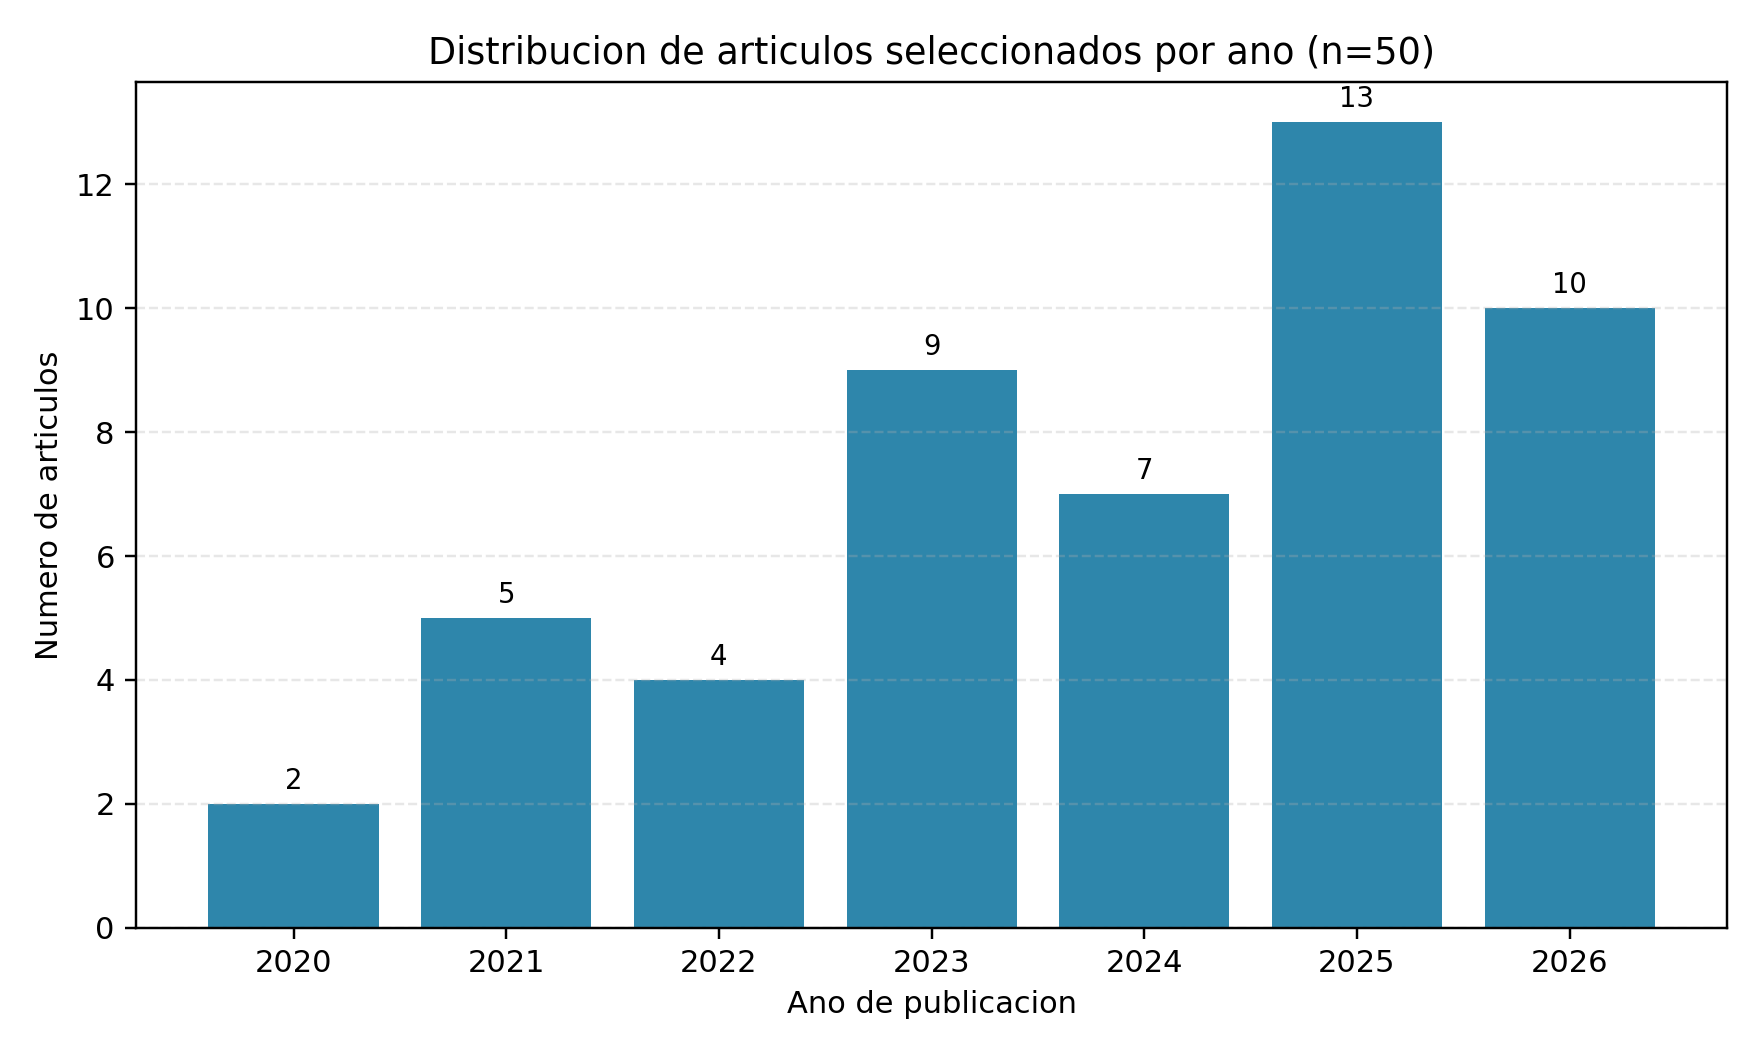
\includegraphics[width=0.9\linewidth]{assets/images/estado_arte_distribucion_anio.png}
    \caption{Distribuci\'on de art\'iculos seleccionados por a\~no (n=50).}
\end{figure}

\begin{figure}[H]
    \centering
    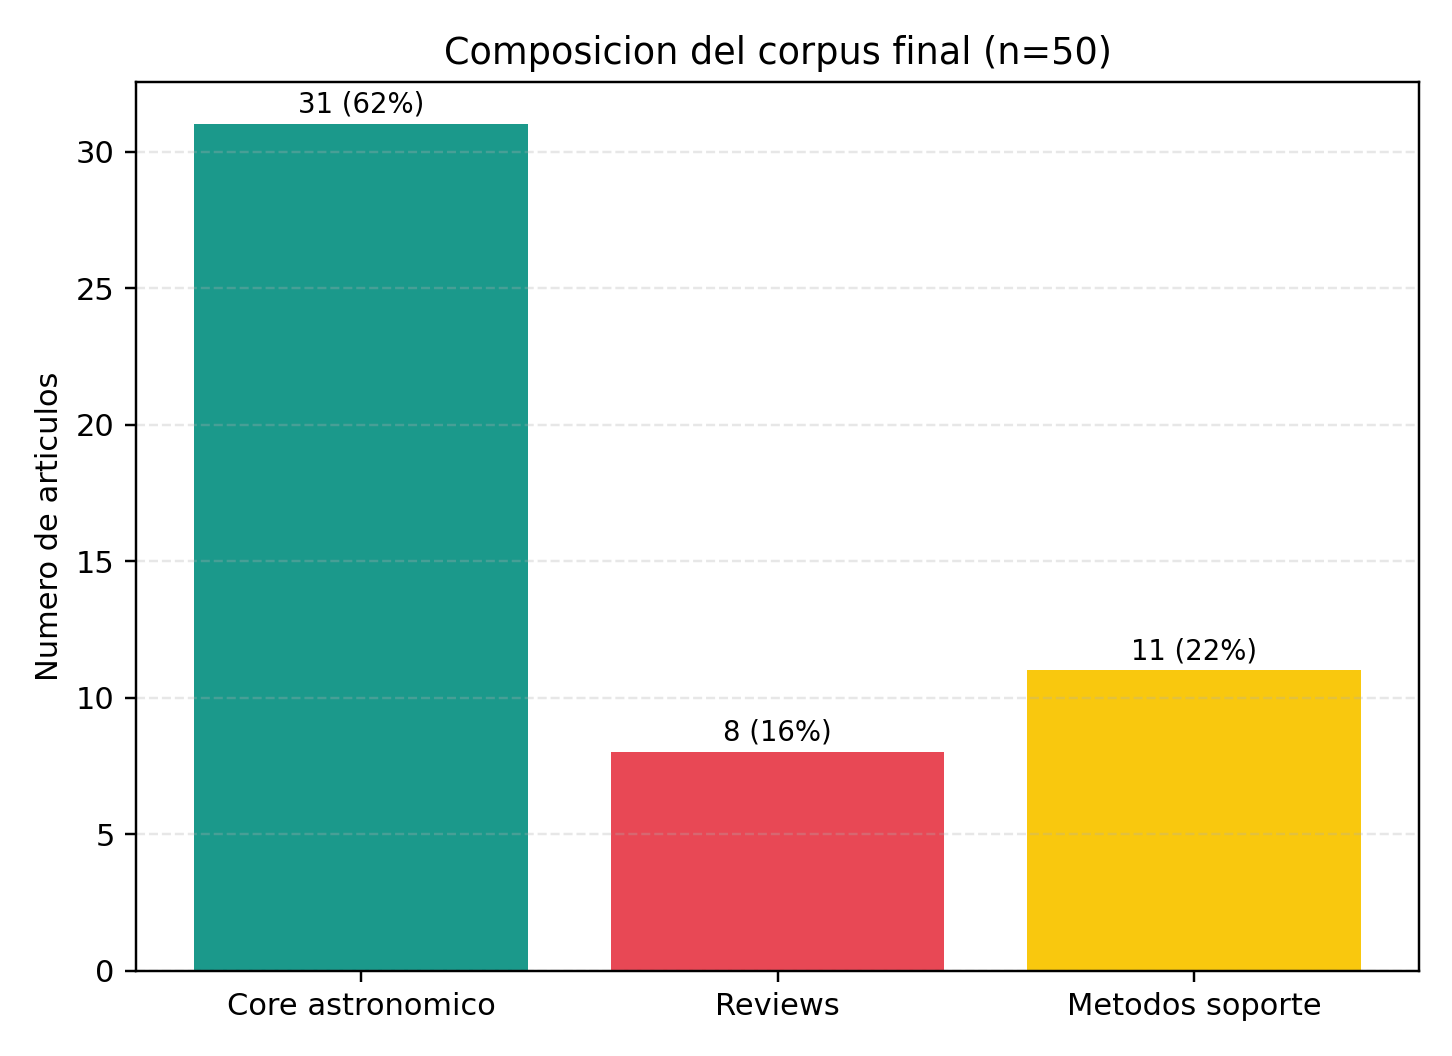
\includegraphics[width=0.8\linewidth]{assets/images/estado_arte_composicion_corpus.png}
    \caption{Composici\'on del corpus final por categor\'ia.}
\end{figure}

\begin{figure}[H]
    \centering
    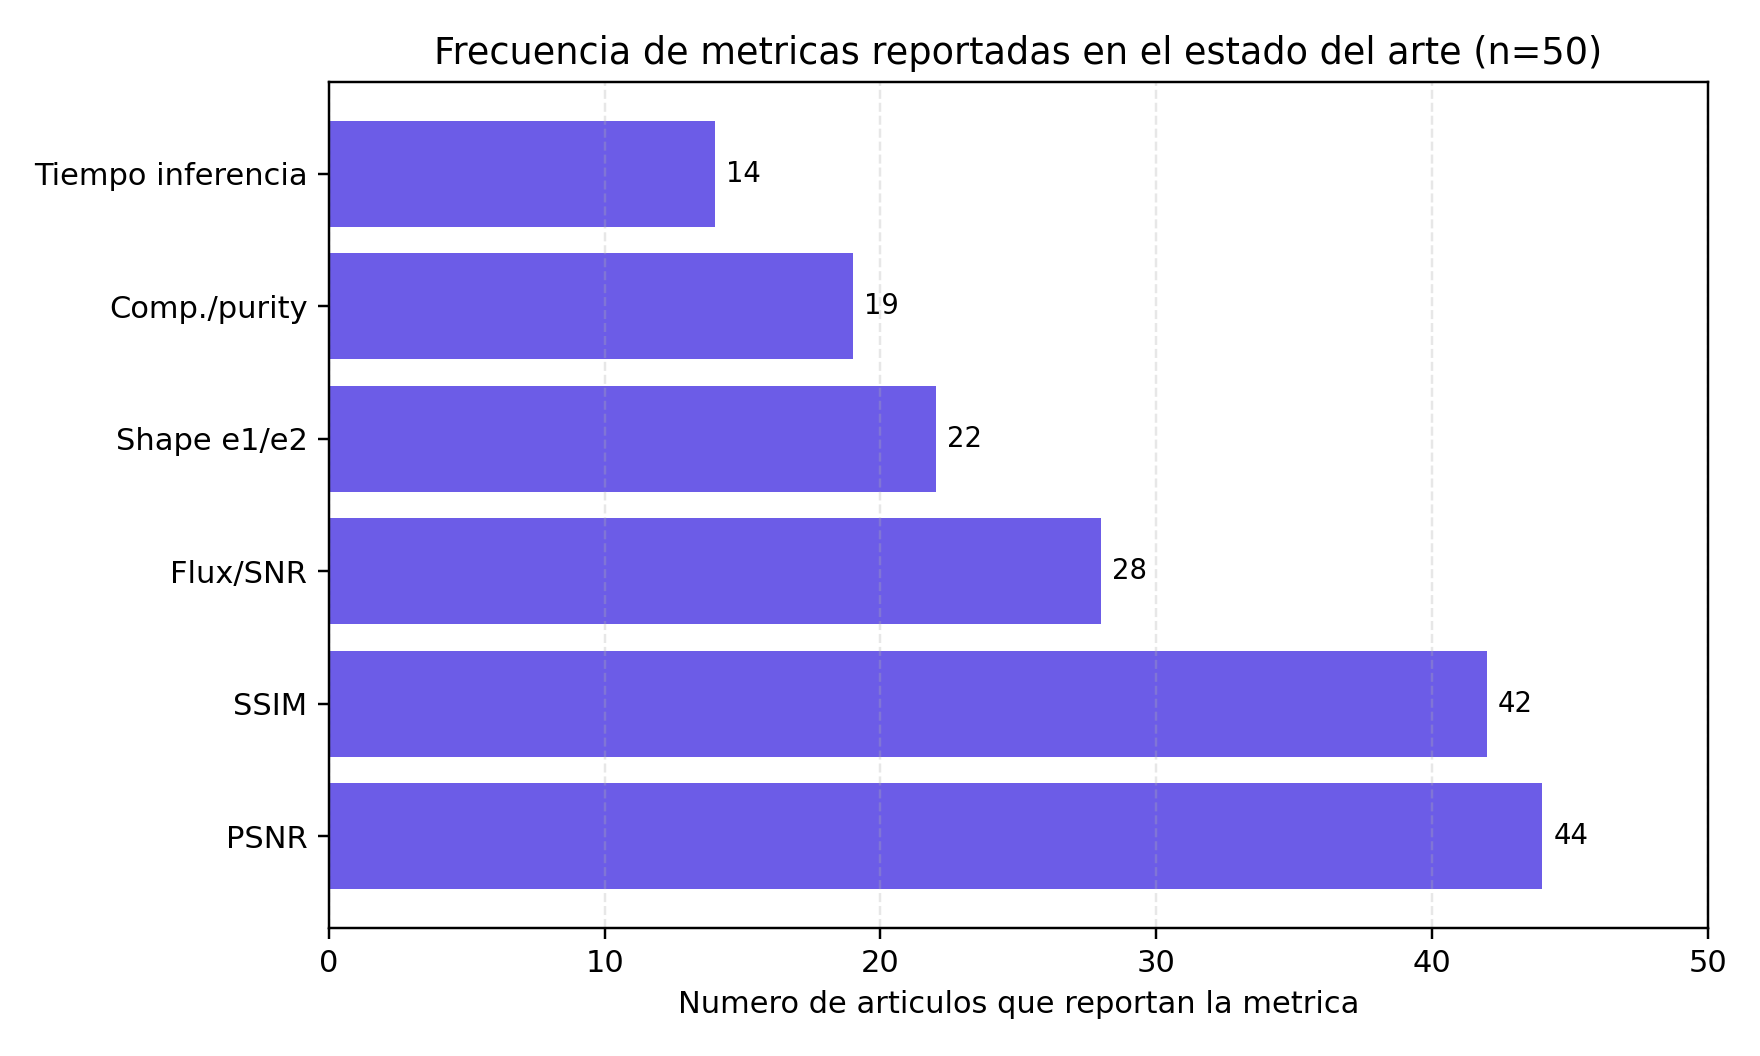
\includegraphics[width=0.9\linewidth]{assets/images/estado_arte_metricas_frecuencia.png}
    \caption{Frecuencia de m\'etricas reportadas en la literatura seleccionada (codificaci\'on cualitativa guiada por RAG + lectura manual).}
\end{figure}

\section{Clasificaci\'on t\'ecnica por enfoques}

\subsection{M\'etodos cl\'asicos y variacionales}
Los enfoques cl\'asicos siguen vigentes como referencia de interpretabilidad y estabilidad, especialmente en escenarios donde el modelo de ruido es conocido o parcialmente controlable \cite{roscani2020comparative, makarkin2021stateart, bui2023poisson}.

\subsection{CNN/U-Net supervisadas}
Las U-Net y variantes contin\'uan siendo un est\'andar de alto rendimiento para restauraci\'on de galaxias y deblending, con mejoras concretas en recuperaci\'on de se\~nal \'util para tareas de cat\'alogo \cite{vojtekova2020unet, hemmati2022deblending, park2024transformer, miao2024astrosr}.

\subsection{Auto-supervisi\'on y entrenamiento sin pares limpios}
Los m\'etodos auto-supervisados reducen la dependencia de datos ``clean'' perfectos, una limitaci\'on cr\'itica en astronom\'ia observacional \cite{liu2025selfsupervised, guo2026detection, sukurdeepa2025astroclearnet}.

\subsection{Modelos generativos y difusi\'on}
La familia de difusi\'on gana tracci\'on por su capacidad de modelar incertidumbre y mejorar escenarios de fondo complejo, incluyendo weak lensing y remoci\'on de ruido de fondo \cite{scognamiglio2025euclid, aoyama2025denoising, nicolaas2025bgrem, schanz2023diffusion, remy2023massmapping}.

\subsection{M\'etodos f\'isica-informados e h\'ibridos}
La integraci\'on de conocimiento instrumental (PSF, ruido CCD, fotometr\'ia multibanda) en arquitecturas profundas se consolida como tendencia de mayor valor para pipelines cient\'ificos robustos \cite{wang2022psf, sreejith2023psf, akhaury2022deep, akhaury2025joint, liu2026ccd}.


\chapter{Justificaci\'on}

\section{Brecha identificada en el marco evaluativo}

La principal brecha identificada no es la falta de modelos de reducci\'on de ruido, sino la ausencia de un marco evaluativo unificado y orientado a validez cient\'ifica. La literatura converge en que la mejora visual no basta y que los costos de validaci\'on ya compiten con el esfuerzo de desarrollo de modelos.

\subsection{Evidencia textual de la necesidad}

\begin{itemize}
    \item Akhaury et al. reportan expl\'icitamente una necesidad metodol\'ogica transversal: \enquote{there is an increasing need to develop fast and accurate deconvolution algorithms that generalize well to different images} \cite{akhaury2022deep}.
    \item Guo et al. muestran el costo operacional de ganar profundidad observacional y justifican alternativas algor\'itmicas: \enquote{improves detection limits by 1.0 magnitude at 90\% completeness and purity} y, para un incremento similar por exposici\'on, se requerir\'ia escalar de d\'ias a cerca de un mes de observaci\'on \cite{guo2026detection}.
    \item En la revisi\'on de Elad et al. se explicita el problema de evaluaci\'on multiojetivo: \enquote{potential solvers need to tradeoff distortion metrics (e.g. MSE) versus perception measures} \cite{elad2023revolution}.
\end{itemize}

\subsection{Implicaci\'on para esta propuesta}

Este proyecto se justifica porque desplaza el centro de gravedad desde \emph{entrenar otro modelo} hacia \emph{establecer una validaci\'on reproducible y con control de sesgo}. En otras palabras, se responde al problema que la comunidad est\'a enfrentando hoy: invertir tiempo de investigaci\'on en dise\~nar marcos de evaluaci\'on comparables, auditables y ligados a impacto cient\'ifico real.

\section{M\'etricas recomendadas para benchmark en LSST/DC2}

Como resultado de la revisi\'on del estado del arte, se propone un marco de validaci\'on en tres capas:

\begin{enumerate}[leftmargin=*]
    \item \textbf{Fidelidad de reconstrucci\'on}: PSNR/SSIM y error de reconstrucci\'on local.
    \item \textbf{Validez cient\'ifica}: completitud-pureza por magnitud, error fotom\'etrico, sesgo en forma (e1/e2), impacto en detecci\'on de fuentes d\'ebiles.
    \item \textbf{Costo operativo}: tiempo de inferencia, estabilidad por dominio y sensibilidad a mismatch de ruido instrumental.
\end{enumerate}

Esta estructura permite comparar m\'etodos heterog\'eneos (cl\'asicos, CNN, difusi\'on, f\'isica-informados) con un mismo criterio de calidad cient\'ifica y no \'unicamente perceptual.

\section{Descripci\'on de datos y materiales}

\subsection{Componentes del dataset}

El dataset de trabajo consiste en dos componentes del release DESC DC2 (dr6-v4) del Vera Rubin Observatory. El primero es \texttt{coadd-t3828-t3829-small}, que contiene im\'agenes coadded de dos tracts del cielo simulado. Una im\'agen coadded es el resultado de apilar m\'ultiples exposiciones, lo que cancela parte del ruido aleatorio pero deja un ruido residual bajo el cual las fuentes d\'ebiles siguen siendo dif\'iciles de detectar.

\bigskip

El segundo componente es \texttt{truth\_match}, el cat\'alogo de verdad de la simulaci\'on, que contiene la posici\'on y el flujo exacto de cada fuente simulada. Este cat\'alogo se utiliza exclusivamente en la etapa de evaluaci\'on para calcular la completitud y pureza de los algoritmos de reducci\'on de ruido.

\subsection{Origen y tama\~nos reales}

A diferencia de las versiones comprimidas, este proyecto trabaja directamente con los archivos en formato FITS para preservar la precisi\'on cient\'ifica total. Los pesos en disco son los siguientes:

\begin{itemize}
  \item \textbf{DESC DC2 Truth Match (\texttt{truth\_match}):} 52 GB (Formato FITS nativo).
  \item \textbf{DESC DC2 Coadded Images (\texttt{coadd-t3828-t3829-small}):} 4.8 GB (Im\'agenes cient\'ificas FITS).
\end{itemize}

\bigskip

\subsection{Flujo del pipeline de procesamiento}

Debido a la complejidad del volumen de datos, se sigue una secuencia estrictamente modular para garantizar la integridad de las m\'etricas:

\begin{mermaid}[width=0.9\linewidth, caption={Secuencia de procesamiento desde datos crudos hasta m\'etricas}, pos=t]
sequenceDiagram
    participant D as Datos (FITS)
    participant P as Preprocesado
    participant A as Algoritmos (BM3D/U-Net)
    participant E as Evaluación (SEP/Metrics)

    D->>P: Carga de HDUs (Ciencia+Varianza)
    P->>P: Sustracción de Fondo + Calibración
    P->>A: Patches de entrada
    A->>E: Imagen procesada (FITS)
    E->>E: Detección de Fuentes
    E->>E: Cross-match con Truth_match
    Note over E: Reporte de Completitud/Pureza
\end{mermaid}

\bigskip

Informaci\'on adicional y documentaci\'on del release: \url{https://data.lsstdesc.org/doc/dc2_sim_sky_survey}.

\bigskip

Los dos componentes mencionados ya han sido descargados y se conservan en el entorno de trabajo para evaluaci\'on reproducible.

\chapter{Metodolog\'ia propuesta}

\section{Resumen}

Este cap\'itulo describe el protocolo experimental propuesto para evaluar m\'etodos de denoising sobre las im\'agenes simuladas DC2 (dr6-v4) del Vera Rubin Observatory. Se prioriza la reproducibilidad absoluta: cada script, semilla aleatoria y log de entrenamiento se registra formalmente para permitir una auditor\'ia completa del proceso.

\section{Flujo experimental}

El flujo general del experimento est\'a diseñado para ser modular y extensible, permitiendo la comparaci\'on justa entre algoritmos de distinta naturaleza:

\begin{mermaid}[width=0.9\linewidth, caption={Secuencia del flujo experimental de benchmarking}, pos=t]
sequenceDiagram
    participant D as Datos (DC2)
    participant P as Preprocesado
    participant M as M\'etodos (BM3D/U-Net)
    participant E as Evaluaci\'on (SEP/Truth)

    D->>P: Carga de Coadds + Truth
    P->>M: Patches normalizados
    M->>E: Imagen Denoised
    E->>E: Detecci\'on + Matching
    Note over E: C\'alculo completitud/pureza
\end{mermaid}

\section{Datos y preprocesado}

Se emplea el release DC2 (espec\'ificamente el tract coadd-t3828-t3829-small) como conjunto principal de entrada. El cat\'alogo \texttt{truth\_match} act\'ua como la ``verdad absoluta'' para evaluar la capacidad de recuperaci\'on de los algoritmos.

El preprocesado incluye la calibraci\'on de unidades, la extracci\'on de parches (patches) representativos y la normalizaci\'on basada en el ruido local. Se presta especial atenci\'on a la conservaci\'on de la PSF (Point Spread Function) local para experimentos de sensibilidad.

\section{M\'etodos a comparar}

En esta fase del proyecto, el benchmark se centra en dos pilares fundamentales que representan el estado del arte cl\'asico y el aprendizaje profundo supervisado:

\begin{itemize}
  \item \textbf{BM3D (Block-matching and 3D filtering):} Seleccionado como el baseline cl\'asico de referencia. Su capacidad para explotar la auto-similitud en la imagen lo hace extremadamente robusto frente a ruidos Gaussianos, aunque su costo computacional es elevado.
  \item \textbf{U-Net (Arquitectura Convolucional Encoder-Decoder):} Representa el enfoque de Deep Learning supervisado. Se entrenar\'a sobre pares de im\'agenes ruidosas/limpias extra\'idas de las simulaciones DC2 para aprender a mapear la estructura gal\'actica subyacente.
\end{itemize}

\section{Protocolo de evaluaci\'on cient\'ifica}

A diferencia de los estudios de visi\'on artificial est\'andar, esta metodolog\'ia prioriza m\'etricas con valor cient\'ifico astron\'omico:

\begin{itemize}
  \item \textbf{Completitud (Recall):} \textquestiondown Qu\'e fracci\'on de las fuentes reales presentes en el catálogo \texttt{truth\_match} somos capaces de detectar tras el denoising?
  \item \textbf{Pureza (Precision):} \textquestiondown Cu\'antas de nuestras detecciones son fuentes reales y no artefactos o ``alucinaciones'' introducidas por el modelo de IA?
  \item \textbf{Precisi\'on Fotom\'etrica:} Medida del bias en la magnitud y el flujo recuperado, asegurando que el denoising no altere la luminosidad intr\'inseca de los objetos.
\end{itemize}

\section{Reproducibilidad y registros}

Para garantizar que cualquier investigador pueda replicar estos resultados, se siguen estrictamente las siguientes pr\'acticas:
\begin{itemize}
  \item Registro de semillas aleatorias en todos los procesos estoc\'asticos.
  \item Uso de contenedores o ambientes virtuales estrictos (\texttt{requirements.txt}).
  \item Generaci\'on autom\'atica de reportes t\'ecnicos que incluyen versiones de software y hardware utilizado.
\end{itemize}

\section{Limitaciones}

Los modelos evaluados no deben haberse entrenado con las regiones del cielo declaradas en la versi\'on del conjunto de datos utilizada; de lo contrario, el resultado del benchmark tendr\'ia sesgo. Por esta raz\'on cada versi\'on del conjunto declara expl\'icitamente sus regiones. La plataforma no puede verificar c\'omo se entren\'o un modelo externo, de modo que el cumplimiento de esta condici\'on depende de la \'etica de cada investigador.

\section{Plan de trabajo y entregables}

Siguiendo el plan de desarrollo establecido, los hitos inmediatos son:

\begin{enumerate}
  \item Implementar y validar el baseline BM3D sobre el dataset DC2 curado.
  \item Entrenar y optimizar la red U-Net supervisada.
  \item Ejecutar el protocolo de comparaci\'on masiva y calcular curvas de completitud vs. pureza.
  \item Publicar el benchmark reproducible con c\'odigo abierto y artefactos de datos.
\end{enumerate}

\paragraph{} Para m\'as detalles t\'ecnicos sobre la arquitectura del orquestador y la evoluci\'on del desarrollo, consulte la \textbf{Hoja de Ruta (Anexo A)} y las \textbf{Especificaciones de Diseño OpenSpec (Anexo B)} al final de este documento.

\chapter{Conclusiones}

\section{Conclusiones sobre el Estado del Arte}

Tras el an\'alisis exhaustivo de la literatura y el proceso de cribado mediante aprendizaje activo, se concluye que el campo de la reducci\'on de ruido en im\'agenes astron\'omicas se encuentra en un punto de inflexi\'on. Mientras que los m\'etodos cl\'asicos como BM3D siguen siendo el est\'andar de oro en cuanto a interpretabilidad f\'isica, las redes neuronales profundas (U-Net) ofrecen una capacidad de recuperaci\'on de señal que supera las t\'ecnicas de filtrado tradicionales en t\'erminos de relaci\'on señal-ruido. Sin embargo, la adopci\'on de IA introduce riesgos de sesgo morfol\'ogico que a\'un no han sido plenamente cuantificados de forma reproducible.

\section{Brechas Detectadas}

A partir de la revisi\'on sistem\'atica, se han identificado las siguientes brechas cr\'iticas que justifican el desarrollo de este benchmark:

\begin{enumerate}
    \item \textbf{Falta de Protocolos Estandarizados:} Existe una disparidad significativa en c\'omo se reportan los resultados de reducci\'on de ruido. Muchos trabajos se limitan a m\'etricas perceptuales (PSNR) sin validar el impacto en el catálogo de fuentes real.
    \item \textbf{Desconexi\'on con la Ciencia Downstream:} Se detecta una necesidad urgente de evaluar si los algoritmos de IA preservan la fotometr\'ia y la morfolog\'ia necesarias para estudios de lente gravitatoria d\'ebil.
    \item \textbf{Dificultad de Reproducci\'on:} Pocos trabajos proporcionan el pipeline completo (scripts de preprocesado + semillas + pesos del modelo), lo que impide la validaci\'on independiente de las mejoras reportadas.
    \item \textbf{Sesgo de Autovalidaci\'on:} Se observa una tendencia recurrente donde los autores proponen simult\'aneamente el modelo y su propio marco de validaci\'on o métricas personalizadas. Esta pr\'actica puede inducir sesgos de confirmaci\'on, ya que las condiciones del experimento suelen estar optimizadas para las fortalezas del algoritmo propuesto, careciendo de un contraste objetivo frente a un estándar externo.
\end{enumerate}


\appendix
\chapter{Hoja de Ruta del Proyecto (\texttt{ROADMAP.md})}

A continuaci\'on se transcribe el plan t\'ecnico y la hoja de ruta establecida para el desarrollo del ecosistema \texttt{astro-denoise}:

\lstinputlisting[basicstyle=\small\ttfamily, breaklines=true, frame=single, caption={Contenido íntegro de ROADMAP.md}]{specs/ROADMAP.md}

\newpage

\chapter{Especificaciones de Diseño (OpenSpec YAML)}

Este anexo contiene las especificaciones t\'ecnicas originales en formato YAML que rigen el desarrollo de los módulos del sistema, referenciadas directamente desde los archivos de definición del proyecto.

\section{Orquestador: \texttt{bench-orquestador-2026.yaml}}
\lstinputlisting[language=bash, basicstyle=\small\ttfamily, breaklines=true, frame=single]{specs/bench-orquestador-2026.yaml}

\section{Baseline BM3D: \texttt{bm3d-baseline-2026.yaml}}
\lstinputlisting[language=bash, basicstyle=\small\ttfamily, breaklines=true, frame=single]{specs/bm3d-baseline-2026.yaml}

\section{Módulo de Métricas: \texttt{metrics-modulo-2026.yaml}}
\lstinputlisting[language=bash, basicstyle=\small\ttfamily, breaklines=true, frame=single]{specs/metrics-modulo-2026.yaml}

\section{Baseline U-Net: \texttt{unet-baseline-2026.yaml}}
\lstinputlisting[language=bash, basicstyle=\small\ttfamily, breaklines=true, frame=single]{specs/unet-baseline-2026.yaml}


  % References
\bibliographystyle{apacite}
\bibliography{bib/all_references}

\end{document}
